% Pursuing Stacks (cotes 134-2 to 134-8): archive cote 134-3, site page 92 (PDF page 93).
% notes for ch. II. Draft compared: ps2.tex:984-1005 ; ps2.tex:1187-1203 ; ps2.tex:1260-1274 ; ps2.tex:1287-1302 ; ps2.tex:1557-1572.
% AI-transcribed by Claude Opus 5.5 (claude-opus-5-5, adaptive thinking, effort high), Message Batches API, batch ps1 (msgbatch_01Rv5hCaNTtUt4JHx1yqoHPL), 2026-11-12; image review recorded in records/CHECK_DECISIONS_134_3_4.tsv.
\scanpage{134-3/92}
\mspage{II iv}

turn out to be irrele\over{\unsure{u}}{v}ant - compare the comme nts in section 26. The re-%
flection on such cellular structures is taken up in section 91, 8$^{\underline{\mathrm{o}}}$ ,
but later again it is kind of superseded by the formalism of ``integrators''
and ``cointegrators''  (in part V of the notes,  on abelianization of homo-%
topy types) which makes a sense in A\hand{\ensuremath{^{\wedge}}}\hand{/} for an arbitrary small category A.

(\hand{!} $^{2\over{\illegible{1}}{2}}$) \xout{Here I am confusing} For a \uline{proper} map of paracompact spaces, thi\over{\illegible{1}}{s}
condition is equivalent \deleted{wi}\over{th}{to} the fibers being ``aspheric'' (i.e. weakly con-%
tractible).

($^{22'}$) This point of view of ``Hot-equivalence classes'' of topologies
is going to lead to the notion\hand{s} of test categories and test functors,
which have proved so hand\over{\unsure{y}}{y} that I did'nt feel later a need to come back
to the former point of view\hand{,} in terms of the understanding  we got with
the test notions.

($^{23}$) We use here the canonical equivalence $B^{\hand{\wedge}}{}_{/a} \hand{\ensuremath{\approxeq}} (B_{/a})^{\hand{\wedge}}$.

($^{24}$) A little later we will say ``test functor'' ins\over[typed]{o}{t}ead of ``\over{a}{e}\over{l}{l}igible
functor'' , and call B a ``test category'' (in a provisional sense, which
\margin{\diagram{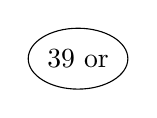
\begin{tikzpicture}[baseline=(n.base)]\node[inner sep=1pt] (n) {39 or};\draw (n.center) ellipse [x radius=1.8em,y radius=1.1em];\end{tikzpicture}}} will be still strengthened somewhat later\over{)}{,} \hand{cf. section} \inserted{39 or} \hand{44).}

($^{25}$) This is now fairly well understood with the notion of an \uline{aspheri-}%
\uline{city structure} (see notably section 77),  and of a ``\uline{canonical modelizer}''
(the idea of which first occurs in section 50).

($^{26}$) See digression in se\over{\unsure{c}}{c}tion 90 on strictly generating families.

($^{27}$) And even without using this topology,  via the obvious functor
$M \hand{\to} B^{\hand{\wedge}}$ \hand{!}

($^{28}$) This reflection on geometric realization is going to stop short,
and the use of the category of topological spaces \inserted{is} fad\over{es}{ing} out altogether.
\hand{(28') This condition will eventually be weakened (\over{\unsure{c}}{c}f. section 41).}

($^{29}$) I did'nt prove yet that (Ord) and (Preord) are modelizers !  I sup-%
pose they are ...

($^{30}$) That these are test categories indeed follows from section 74,
and it is equally true that the natural functors from these into (Cat)\hand{\begin{tikzpicture}[x=.8em,y=.8ex,baseline=-.3ex]\draw (.6,.65)--(0,.35)--(.42,.05);\draw (.56,-.05)--(.18,-.25) .. controls (-.03,-.48) and (.25,-.76) .. (.33,-.56);\end{tikzpicture}}
\hand{(}used below in order to describe the functors $\hand{\ensuremath{\alpha}}_{p,q}$\hand{)} are test functors
(cf. remark after the proof of prop.2 in section 82),  and therefore
$\hand{\ensuremath{\alpha}}_{p,q}$ is indeed modelizing.

($^{31}$) However \hand{\ensuremath{\mathord{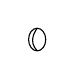
\begin{tikzpicture}[x=1ex,y=1ex,baseline=-.5ex]\draw (0,0) ellipse (.72 and .95);\draw (0,-.95) .. controls (-.75,-.15) and (-.2,.65) .. (0,.95);\end{tikzpicture}}}} (compare note ($^4$)) is more economical still !

($^{32}$) I am not sure that the passage through semisimplicial formalism,
for describing a $\overset{\hand{\vee}}{\mathrm{C}}$ech-Cartier-Verdier \over{formalism}{functor}\hand{,} is the most efficient way\hand{,}

\mspage{\hand{92}}
